%\documentclass[11pt,twoside,a4paper]{article}
\documentclass[11pt,a4paper]{article}
\usepackage[italian]{babel}
\usepackage{listings}
\usepackage{color}
\usepackage{mathtools}
\usepackage{biblatex}
\usepackage{float}

%useful colors
\definecolor{mygreen}{rgb}{0,0.6,0}
\definecolor{mygray}{rgb}{0.5,0.5,0.5}
\definecolor{mymauve}{rgb}{0.58,0,0.82}
\definecolor{gray}{rgb}{0.4,0.4,0.4}
\definecolor{darkblue}{rgb}{0.0,0.0,0.6}
\definecolor{cyan}{rgb}{0.0,0.6,0.6}
%defining styles for listings
%java listings
\lstdefinestyle{java}{
	basicstyle=\footnotesize,
	breakatwhitespace=false,
	breaklines=true,
	captionpos=b,
	commentstyle=\color{mygreen},
	frame=single,
	keywordstyle=\color{blue},
	language=java,
	numbers=left,
	numbersep=5pt,
	numberstyle=\tiny\color{mygray},
	rulecolor=\color{black},
	showstringspaces=false,
	stepnumber=1,
	stringstyle=\color{mymauve},
	tabsize=2,
	title=\lstname
}
%javascript listings
\lstdefinestyle{javascript}{
	basicstyle=\footnotesize,
	breakatwhitespace=false,
	breaklines=true,
	captionpos=b,
	commentstyle=\color{mygreen},
	frame=single,
	keywordstyle=\color{blue},
	language=javascript,
	numbers=left,
	numbersep=5pt,
	numberstyle=\tiny\color{mygray},
	rulecolor=\color{black},
	showstringspaces=false,
	stepnumber=1,
	stringstyle=\color{mymauve},
	tabsize=2,
	title=\lstname
}
%php listings
\lstdefinestyle{php}{
	basicstyle=\footnotesize,
	breakatwhitespace=false,
	breaklines=true,
	captionpos=b,
	commentstyle=\color{mygreen},
	frame=single,
	keywordstyle=\color{blue},
	language=php,
	numbers=left,
	numbersep=5pt,
	numberstyle=\tiny\color{mygray},
	rulecolor=\color{black},
	showstringspaces=false,
	stepnumber=1,
	stringstyle=\color{mymauve},
	tabsize=2,
	title=\lstname
}
%xml listings
\lstdefinelanguage{XML}
{
	morestring=[b]",
	morestring=[s]{>}{<},
	morecomment=[s]{<?}{?>},
	stringstyle=\color{black},
	identifierstyle=\color{darkblue},
	keywordstyle=\color{cyan},
	morekeywords={xmlns,version,type}% list your attributes here
}


\lstdefinestyle{xml}{
	basicstyle=\ttfamily,
	breakatwhitespace=false,
	breaklines=true,
	columns=fullflexible,
	showstringspaces=false,
	captionpos=b,
	commentstyle=\color{mygreen},
	frame=single,
	keywordstyle=\color{blue},
	language=XML,
	numbers=none,
	rulecolor=\color{black},
	tabsize=4,
	title=\lstname
}
\begin{document}
\title{Finding similar papers using ontologies}
\author{Francesco Gaetano, Luigi Lomasto, Marco Mecchia, Andrea Sold\'a }
\date{Gennaio 2016}
\maketitle
\section{Introduzione al problema}
Il problema di trovare lavori scientifici simili scritti in linguaggio naturale \'e un compito molto difficile dal punto di vista informatico: Tali documenti infatti non hanno una struttura fissa, e sono pieni  di elementi non facilmente confrontabili come formule, notazioni ed immagini. Inoltre, nonostante una netta predominanza dell'inglese, i documenti sono scritti in lingue diverse. Tutte queste caratteristiche, insite in lavori di ricerca di questo tipo, rendono gli approcci basati sul confronto testuale non utilizzabili. Il nostro lavoro, basato sulle meta informazioni dei documenti e sull'utilizzo di tecnologie del Semantic Web, mira a fornire un approccio alternativo ai metodi tradizionali, nonch\'e un'infrastruttura riutilizzabile anche in altri ambiti.

Il resto del lavoro \'e organizzato come segue: nella sezione \ref{sec:workflow} viene presentata l'analisi da noi condotta ed i vari step che hanno portato al risultato finale. Nella sezione \ref{sec:tools} vengono analizzati nel dettaglio le tecnologie del Web Semantico da noi utilizzate. Nella sezione \ref{sec:implementation} vengono presentate nel dettaglio le varie componenti introdotte nella sezione \ref{sec:workflow}, illustrando e commentando estratti di codice del progetto. Infine, nella sezione \ref{sec:conclusions} verranno commentati i risultati ottenuti ed eventuali applicazioni ed estensioni di quanto fatto.

\section{Workflow}
\label{sec:workflow}
Il lavoro \'e stato suddiviso in diverse fasi. 

\subsection{Selezione del database ed estrazione delle meta-informazioni}
\label{subsec:infoextraction}
In questa fase preliminare del lavoro, abbiamo costruito il dataset sul quale basarci per tutto il resto del lavoro. Per prima cosa abbiamo scelto il database dal quale attingere i lavori da confrontare. La nostra scelta e' ricaduta su DBLP\cite{DBLP} in quanto punto di riferimento centrale per la sottomissione dei paper nella comunita' informatica. DBLP inoltre mette a disposizione ampi dataset di meta-informazioni sugli articoli scaricabili in formato standard xml, con relativi url alle pagine web degli articoli.
Mediante gli url letti dal file dblp.xml, per ogni articolo abbiamo estratto dalla pagina sorgente l'abstract ed eventualmente topics e keywords (se presenti). Questo lavoro ci ha permesso di ottenere un primo dataset che, oltre alle informazioni di partenza, contiene anche gli abstract con eventuali topics o keywords. Poich\'e topics e keywords sono state estratte dalla pagina sorgente dell'articolo, \'e stato deciso di assegnare, per ogni topic una relevance pari ad 1, e per ogni keyword una relevance pari a 0.99.\newline \newline
A partire da questa prima versione, con l'utilizzo delle API di Alchemy abbiamo, per ogni abstract, estratto le keywords con le rispettive relevance, ottenendo cos\'i il dataset finale, sostituendo all'abstract le keywords ottenute. Il dataset finale contiene per ogni articolo le seguenti informazioni:

\begin{itemize}
	\item Titolo del lavoro
	\item Autori del lavoro
	\item Anno di pubblicazione
	\item Topics (se presenti)
	\item Keyword (se presenti)
	\item Rivista
	\item URL
\end{itemize} 


\subsection{Progettazione e popolamento dell'ontologia}
\label{subsec:ontology}
In questa fase, \'e stata studiata la progettazione di un'ontologia adatta a gestire le informazioni estratte nella fase precedente. Il passaggio ad un'ontologia \'e stato necessario per almeno due motivi:
\begin{enumerate}
	\item La possibilit\'a di interrogare il database di meta informazioni tramite query semantiche.
	\item La possibilit\'a di collegare il lavoro a strumenti gi\'a esistenti per i \emph{linked data}, in modo da rendere lo strumento integrabile.
\end{enumerate}
Per l'ontologia, la nostra scelta \'e ricaduta su CIDOC/CRM\cite{CIDOC}. Il modello concettuale CIDOC/CRM \'e un stato progettato per la gestione di contenuti relativi alla storia ed alle opere d'arte, quindi si \'e rivelato adatto al nostro scopo. 




-----------Qui c\'e da appronfondire sullo schema che abbiamo progettato noi a partire dalle meta informazioni Francesco-----

\subsection{Interrogazione dell'ontologia}
\label{subsec:query}
Una volta popolata l'ontologia \'e stata necessaria la progettazioni di query adatte al contesto del progetto. Le query su cui \'e stata dedicata maggiore attenzione sono due:
\begin{enumerate}
	\item A partire dal titolo di un articolo, restituire  keywords e topics.
	\item A partire da keywords e topic ottenuti dalla query precedente, restituire la lista degli articoli che hanno un'sottoinsieme di keywords e topics in comune. 
	\item A partire dal titolo di un articolo, restituire tutte le informazioni quali: Autori, anno di pubblicazione, rivista, url ...
\end{enumerate}

\subsection{Presentazione dei risultati}
\label{subsec:results}

Una volta progettate ed eseguite le query, abbiamo studiato un modo per poter proporre i risultati in modo elegante, ma che allo stesso tempo ponesse enfasi sullo strato semantico che lega i documenti. Per fare ci\'o, abbiamo generato in maniera ricorsiva un grafo centralizzato: la radice \'e il documento di partenza, ed il solo nodo presente nel grafo. Il livello $i+1$-esimo del grafo viene generato semplicemente lanciando la query principale su tutti gli articoli del livello $i$-esimo. Il processo viene reiterato finch\'e non si arriva alla profondit\'a desiderata.

\section{Strumenti utilizzati}
\label{sec:tools}
Le tecnologie utilizzate per lo sviluppo di questo progetto sono molteplici:
\begin{itemize}
	\item Java 8 per gran parte del backend, cio\'e lo scraping e la popolazione dell'ontologia. Abbiamo usato le seguenti librerie:
	\begin{itemize}
		\item jsoup per l'utilizzo di espressioni Xpath nella fase di scraping.
		\item Apache Jena per la popolazione dell'ontologia e la creazione del file .owl.
		\item AlchemyAPI per l'estrazione delle keywords da ogni topic.
	\end{itemize}
	\item Abbiamo utilizzato le seguenti tecnologie del Semantic Web:
	\begin{itemize}
		\item Protege per creare ed estendere lo schema ontologico.
		\item OWL come linguaggio per definire l'ontologia.
		\item SPARQL come linguaggio di query per interrogare l'ontologia.
		\item Apache Fuseki come server per gestire le query.
	\end{itemize}
	\item PHP7 per la formulazione e la sottomissione delle query lato server.
	\item Javascript per la parte di frontend, utilizzando le seguenti librerie:
	\begin{itemize}
		\item vis.js per il rendering del grafo.
		\item JQuery per gestire meglio le richieste ajax agli script Php lato server.
		\item Bootstrap per la gestione dell'aspetto della pagina.
	\end{itemize}
\end{itemize}

\subsection{Jsoup}
Libreria Java che permette di lavorare con documenti HTML. Fornisce delle API molto semplici con le quali \'e possibile estrarre e manipolare i dati a partire dal DOM di una pagina mediante l'uso di espressioni XPath. 
\newline \newline 
\textbf  {Esempio}
\begin{lstlisting}[breaklines=true]
Document doc = Jsoup.connect(URL).timeout(50*1000).get();
Elements elemsAbstract = doc.select("p.Para");
\end{lstlisting} 

\subsection{Prot\'eg\'e}
Prot\'eg\'e \'e un framework open source sviluppato presso l'universit\'a di Stanford, esso dispone di un'interfaccia grafica per la definizione di schemi ontologici e della semantica alla base di essi. Tramite il tool \'e stato possibile importare lo schema ontologico tipico di CIDOC-CRM sulla quale successivamente si \'e reso necessario la definizione di classi e proprietà supplementari per estendere lo schema in uno maggiormente adatto per la nostra applicazione.

\subsection{Apache Jena}
Apache Jena è un framework open source per Java, il quale fornisce API per la lettura e scrittura di grafi RDF. In particolare, \'e stato utilizzato per la lettura dello schema precedentemente realizzato con Prot\'eg\'e e per la successiva scrittura di uno schema OWL comprendente le istanze a partire da un dataset in input.

\subsection{AlchemyAPI}
AlchemyAPI utilizza algoritmi per  l'apprendimento automatico che permettono di  estrarre meta-dati semantici dal contenuto desiderato, come ad esempio informazioni su persone, luoghi, aziende, gli argomenti, i fatti, le relazioni, gli autori e le lingue. I meta-dati possono essere restituiti in formato XML, JSON e RDF. \newline
Ad ogni parola estratta viene associato una relevance (valore numerico compreso tra 0 e 1), che indica l'incidenza della parola all'interno del testo.
Nel nostro caso sono state usate parole con relevance maggiore o uguale di 0.6. 

\subsection{Vis.js}
Vis.js \'e una libreria javascript che permette la visualizzazione dinamica di grafi, timeline e grafici a due o tre dimensioni. La struttura architetturale \'e illustrata nell'immagine seguente.
\begin{figure} [!h] 
\centering
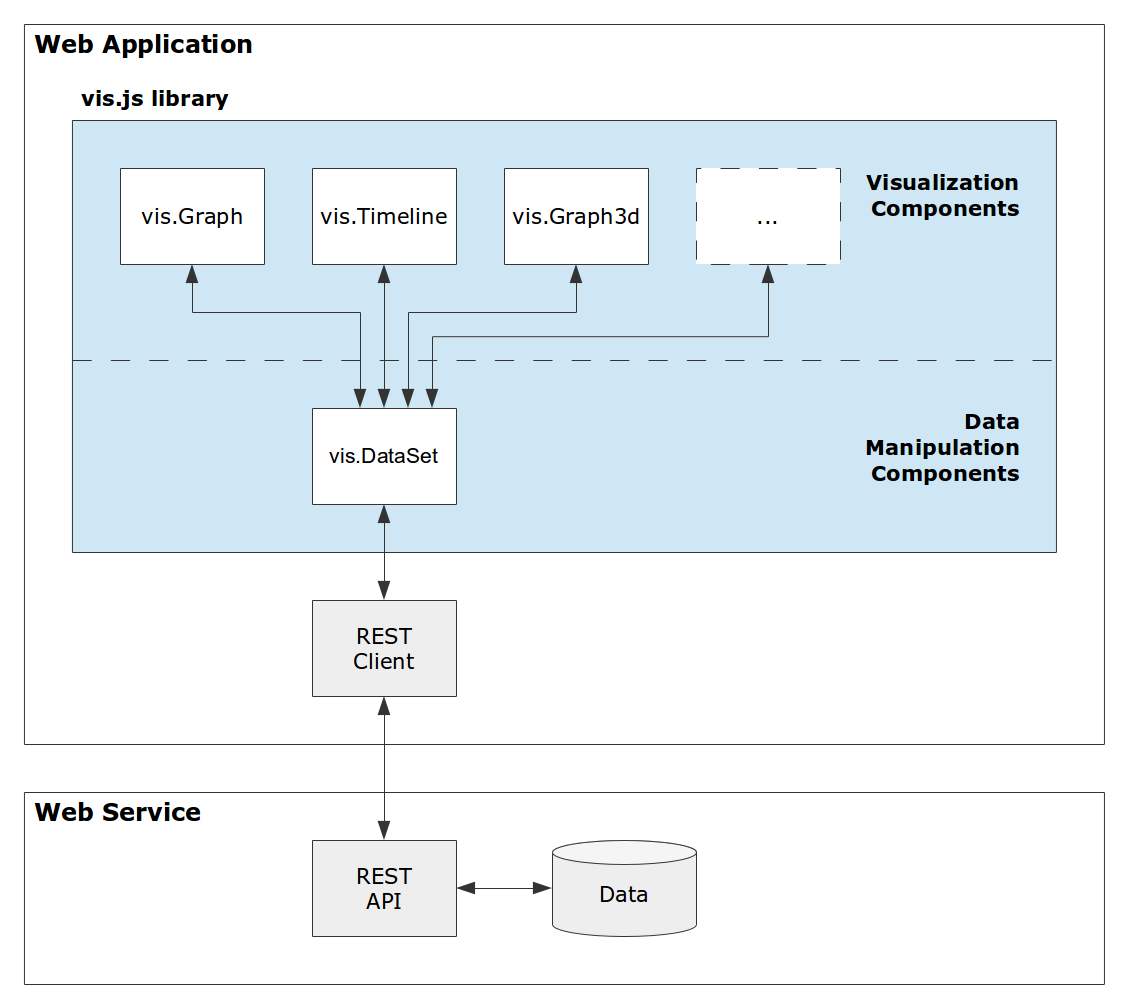
\includegraphics[scale=0.45]{immaginiTesina/vis_overview.png}
\end{figure}


Nel nostro caso abbiamo usato tale libreria per generare un grafo contenete gli articoli con le relative relazioni semantiche. Un grafo in Vis.js \'e una struttura costituita da nodi ed archi. Di seguito \'e riportato un esempio con cinque nodi e quattro archi.

\begin{lstlisting}[breaklines=true]
<!doctype html>
<html>
<head>
  <title>Network | Basic usage</title>

  <script type="text/javascript" src="../../dist/vis.js"></script>
</head>

<body>

<div id="mynetwork"></div>

<script type="text/javascript">
  // create an array with nodes
  var nodes = [
    {id: 1, label: 'Node 1'},
    {id: 2, label: 'Node 2'},
    {id: 3, label: 'Node 3'},
    {id: 4, label: 'Node 4'},
    {id: 5, label: 'Node 5'}
  ];

  // create an array with edges
  var edges = [
    {from: 1, to: 2},
    {from: 1, to: 3},
    {from: 2, to: 4},
    {from: 2, to: 5}
  ];

  // create a network
  var container = document.getElementById('mynetwork');
  var data= {
    nodes: nodes,
    edges: edges,
  };
  var options = {
    width: '400px',
    height: '400px'
  };
  var network = new vis.Network(container, data, options);
</script>

</body>
</html>
\end{lstlisting}


\section{Implementazione}
\label{sec:implementation}


\subsection{Costruzione del dataset}
Per costruire il dataset di meta-informazioni dei documenti presenti su DBLP, \'e stato sviluppato un package java chiamato \emph{scraper}, costituito dalle seguenti classi:
\begin{description}
	\item[.java] Contenente il main. Si occupa, preso in input il dataset di meta-informazioni degli articoli scaricabile da DBLP, di eliminafare le informazioni superflue e di invocare le classi di scraping quando si trova l'elemento <url>.
	\item[SuperScraper.java] Superclasse astratta degli scraper, utile per il polimorfismo.
	\item[FactoryScraper.java] Implementazione del Factory Method per gli scraper.
	\item[IJIEMScraper.java] Istanza di SuperScraper.
	\item[JDisplaScraper.java] Istanza di SuperScraper.
	\item[JkdbScraper.java] Istanza di SuperScraper.
	\item[StandardScraper.java] Istanza di SuperScraper.
\end{description}

\paragraph{Count}
\label{par:count}

\lstinputlisting[style=java, firstline=10, caption=Count.java]{./src/Count.java}

Il main prende due argomenti da linea di comando: il primo corrisponde al percorso del file xml di informazioni di DBLP, ed il secondo al nome del file dove ricopiare il dataset aggiornato. Il cuore della classe \'e costituito dal metodo statico parsing: Tale metodo legge il file XML riga per riga, fino a trovare la riga contentente l'URL dell'articolo; una volta trovato, la factory crea uno scraper apposito in base al contenuto della linea. Lo scraper si occupa di effettuare la connessione all'url, di estrarre l'abstract dalla pagina web e di aggiornare il file di output. Grazie al Factory Method ed al polimorfismo, aggiungere nuovi scraper e' semplicissimo, e non richiede l'intervento diretto sul main. Il numero di articoli \'e stato impostato a 5000 poich\'e tale numero si \'e rivelato sufficiente per costruire il nostro dataset.

\paragraph{StandardScraper}
\label{par:standardscraper}
La classe StandardScraper \'e un'istanza della superclasse SuperScraper, e si occupa di scrivere in output le informazioni estratte da un articolo in un file xml.
\lstinputlisting[style=java, firstline=16, caption=StandardScraper.java]{./src/scraper/StandardScraper.java}

Questo tipo di output e' lo stesso per tutte le istanze degli scraper. Quello che differenzia ogni scraper \'e la struttura della pagina che vanno ad esaminare, per cui sono richiesti controlli ed espressioni Xpath diverse per estrarre le informazioni giuste. Se il documento contiene delle keyword, esse vengono aggiunte in un apposito tag dopo i topic, prima della chiusura del tag relativo all'articolo.

\lstinputlisting[style=xml, firstline=4, lastline=21, caption=Esempio di xml prodotto dallo StandardScraper]{./lib/datasetWithAbstract/dataset1.xml}

\paragraph{FactoryScraper}
\label{par:factoryscraper}

\lstinputlisting[style=java, firstline=3, caption=FactoryScraper.java]{./src/scraper/FactoryScraper.java}

La FactoryScraper alla sua creazione crea un tipo di oggetto per ogni specializzazione della classe SuperScraper; in questo modo, quando c'\'e bisogno di fare il parsing di un nuovo documento non si crea ogni volta un nuovo oggetto, ma si utilizza sempre lo stesso. Cos\'i facendo, gli oggetti vengono riutilizzati e vengono risparmiati memoria e processore, in quanto la Garbage Collector di Java non deve essere invocata di continuo. Il metodo createScraper si deve solamente occupare di verificare le condizioni per cui deve essere creato un tipo di Scraper piuttosto che un altro.

\subsection{Estrazione delle Keyword}
Per l'estrazione delle keyword a partire dall'abstract \'e stato fatto uso delle API messe a disposizione dal software Alchemy\cite{alchemy}, scaricabili gratuitamente. Tale software \'e composto da molti strumenti utili per l'analisi linguistica, tra cui l'estrazione di parole chiave da un testo con rilevanze normalizzate nell'intervallo $[0,1]$. Gli unici limiti riscontrati sono stati il fatto di doversi registrare per ottenere una chiave per utilizzare le API ed il relativo limite di chiamate giornaliere.

Il pacchetto \emph{keyword} sviluppato nel progetto \'e composto da due classi:
\begin{description}
	\item[KeywordExtractor] \'e una classe di wrapper per la chiamata al metodo di AlchemyAPI che dato un testo restituisce le keyword rankate.
	\item[ScraperForKeyword] \'e la classe contentente il metodo main del pacchetto. Si occupa di aggiungere al dataset generato con il pacchetto scraper le keyword estratte con la classe KeywordExtractor.
\end{description}

\paragraph{ScraperForKeyword}
\label{par:scraperforkeyword}

\lstinputlisting[style=java, firstline=21 caption=ScraperForKeyword.java]{./src/keywords/scraperForKeyword.java}

Il main prende in input 5 argomenti: il numero di articoli gi\'a letti, il numero di articoli da leggere, il percorso del file di input\footnote{Nel file ci sono gi\'a gli abstract, estratti con il pacchetto scraper.}, il percorso del file di output ed il percorso della chiave per utilizzare le API di Alchemy. Il numero di articoli gi\'a letti e quelli da leggere sono parametri necessari introdotti dal limite di chiamate di AlchemyAPI; in questo modo il lavoro \'e stato diviso tra i componenti del team in maniera facilmente ricostruibile.

Dopo aver saltato gli articoli gi\'a letti, il parser per ogni articolo trova l'abstract ed esegue una chiamata al metodo statico ExtractKeyword della classe KeywordExtractor. Grazie al metodo di utilit\'a getStringFromDocument, il documento xml contenente le keyword dell'abstract viene serializzato. La stringa corrispondente al documento serializzato a questo punto viene concatenata alle informazioni del documento e viene quindi scritta in output.

\paragraph{KeywordExtractor}
\label{par:keywordextractor}
La classe \'e composta dal solo metodo statico ExtractKeyword. Tale metodo prende in input il testo da cui estrarre le parole chiave ed il percorso del file contenente la chiave fornita dal sito web di Alchemy. Il metodo restituisce un documento xml sotto forma di oggetto Document; in questo modo \'e facilmente serializzabile, oltre che navigabile con gli strumenti del DOM.

\lstinputlisting[style=java, firstline=13, caption=KeywordExtractor.java]{./src/keywords/KeywordExtractor.java}


\lstinputlisting[style=xml, caption=Esempio di documento restituito dalla classe KeywordExtractor]{alchemyexemple.xml}

\subsection{Lo schema ontologico}
Una volta realizzato il dataset con le relative informazioni, il passo successivo è stato quello di definire la semantica sottostante. L'idea è stata quella di partire da uno schema esistente che fosse flessibile per avere l'opportunità di estenderlo nel caso fosse stato necessaria l'aggiunta di ulteriori entit\'a.

\subsubsection{Conceptual Reference Model (CRM);}
Il modello utilizzato è il CIDOC-CRM, usato da musei ed altre istuzioni culturali per la descrizione di relazioni tra entità per valorizzare lo scambio di informazioni tra fonti eterogenee.
 
Per definizione, un'onotologia \'e CRM compatibile se rispetta lo schema di base proposto dagli autori.

 Lo schema di base attualmente comprende  93 classi e 165 proprietà delle quali solo un sottoinsieme sono risultate funzionali al nostro obiettivo:
	 \begin{itemize}
	 	\item Entit\'a
	 	\begin{enumerate}
	 		\item \textbf{E1\_Production:} In CRM un oggetto reale è opportuno vederlo come il risultato di un'attività (in questo l'attività è descritta come "produzione"). Nel nostro caso un qualsiasi articolo può essere visto come il prodotto risultante
	 	\end{enumerate}
	 \end{itemize}
 
 Per rappresentare in modo corretto le informazioni estratte da DBLP \'e stato necessario aggiungere, allo schema di base del CRM, altre classi e propriet\'a. 
  
\begin{center} 
	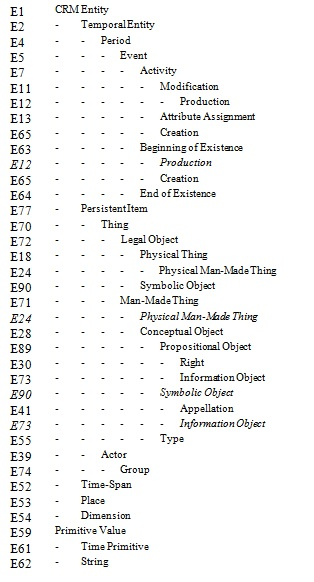
\includegraphics[scale=1.50]{immaginiTesina/ridotto.jpg}
\end{center}

\subsubsection{Estensioni al CRM}
Essendo un modello principalmente progettato per le istituzioni culturali, è stato necessario effettuare delle aggiunte allo schema di partenza. Di seguito verrano elencate le entità e le proprietà con le opportune motivazioni:
%\begin{itemize}
%	\item Entità
		%\begin{enumerate}
			%contenuto...
		%\end{enumerate}
%\end{itemize}

\subsection{Popolamento dell'ontologia}


\subsection{Query SPARQL}

Per poter effettuare al meglio le query sull'ontologia abbiamo deciso di implementare la classe \textit{query-sparql} (file query.php). Tale classe è costituita da funzioni che, quando chiamate, restituiscono la query ad esse associate.
\newline \newline
La lista degli articoli che contengono un sottoinsieme di keywords e topics dei medesimi dell'articolo di partenza, viene resituita in formato JSON dal file ricerca.php all'interno del quale vengono fatte le chiamate a funzione della classe \textit{query-sparql}. Il JSON restituito \'e un array contenente la lista di keywords e topics dell'articolo di partenza e da un array contenete oggetti di tipo \textit{article} dove per ognuno è riportata la lista di keyword e topic che corrispondono, il titolo e l'id che identifica univocamente il nodo del grafo successivamente associato.
Di seguito sono riportate alcune delle query  Sparql usate per interrogare l'ontologia. Per ulteriori chiarimenti consultare i file query.php e ricerca.php.

\begin{itemize}
\item \textbf{Dal titolo di un articolo estrarre topic.}
\begin{lstlisting}[breaklines=true]
prefix crm: <http://www.cidoc-crm.org/cidoc-crm/>
prefix owl: <http://www.w3.org/2002/07/owl#>
prefix sd: <http://www.semanticweb.org/francesco/ontologies/2016/docs#>

SELECT  ?title_value ?topic_value
 
  WHERE{
  ?prod crm:P108_has_produced ?doc.
  ?doc crm:P102_has_title ?title.
  ?title sd:Title_value "Representation of Graphs".
  ?title sd:Title_value ?title_value.
  ?doc crm:P56_bears_feature ?topic.
  ?topic sd:Topic_value ?topic_value.
}
\end{lstlisting}
\end{itemize}

\begin{itemize}
\item \textbf{Dal titolo di un articolo estrarre keywords e relevance.}
\begin{lstlisting}[breaklines=true]
prefix crm: <http://www.cidoc-crm.org/cidoc-crm/>
prefix owl: <http://www.w3.org/2002/07/owl#>
prefix sd: <http://www.semanticweb.org/francesco/ontologies/2016/docs#>

SELECT  ?title_value ?t ?r
 
  WHERE{
  ?prod crm:P108_has_produced ?doc.
  ?doc crm:P102_has_title ?title.
  ?title sd:Title_value "Representation of Graphs".
  ?title sd:Title_value ?title_value.
  ?doc crm:P149_is_identified_by ?key.
  ?key sd:Text ?t.
  ?key sd:Relevance ?r
}
\end{lstlisting}
\end{itemize}

\begin{itemize}
\item \textbf{Dalle keywords dell'articolo di partenza estrae gli articoli che hanno un sottoinsieme di keyword in comune, escludendo l'articolo di partenza.}
\begin{lstlisting}[breaklines=true]
prefix crm: <http://www.cidoc-crm.org/cidoc-crm/>
prefix owl: <http://www.w3.org/2002/07/owl#>
prefix sd: <http://www.semanticweb.org/francesco/ontologies/2016/docs#>
prefix xsd: <http://www.w3.org/2001/XMLSchema#>


SELECT   ?title_value  (SUM(xsd:double(?r)) as ?totalR) 

WHERE
{
  {?prod crm:P108_has_produced ?doc.
  ?doc crm:P102_has_title ?title.
  ?title sd:Title_value ?title_value.
  ?doc crm:P149_is_identified_by ?key.
  ?key sd:Relevance ?r.
  ?key sd:Text ?t.
    FILTER(?t="following sense")} UNION 
  {?prod crm:P108_has_produced ?doc.
  ?doc crm:P102_has_title ?title.
  ?title sd:Title_value ?title_value.
  ?doc crm:P149_is_identified_by ?key.
  ?key sd:Relevance ?r.
  ?key sd:Text ?t.
    FILTER(?t="transition systems")} UNION
  {?prod crm:P108_has_produced ?doc.
  ?doc crm:P102_has_title ?title.
  ?title sd:Title_value ?title_value.
  ?doc crm:P149_is_identified_by ?key.
  ?key sd:Relevance ?r.
  ?key sd:Text ?t.
    FILTER(?t="label-disjoint cycles")}UNION
  {?prod crm:P108_has_produced ?doc.
  ?doc crm:P102_has_title ?title.
  ?title sd:Title_value ?title_value.
  ?doc crm:P149_is_identified_by ?key.
  ?key sd:Relevance ?r.
  ?key sd:Text ?t.
    FILTER(?t="finite labelled transition")}UNION
   {?prod crm:P108_has_produced ?doc.
  ?doc crm:P102_has_title ?title.
  ?title sd:Title_value ?title_value.
  ?doc crm:P149_is_identified_by ?key.
  ?key sd:Relevance ?r.
  ?key sd:Text ?t.
    FILTER(?t="finite set")}
  
  FILTER(?title_value!="A decomposition theorem for finite 
  persistent transition systems").
}

group by ?title_value
ORDER BY DESC(?totalR) 
\end{lstlisting}
\end{itemize}


\begin{itemize}
\item \textbf{Dai topics dell'articolo di partenza estrae gli articoli che hanno un sottoinsieme di topic in comune, escludendo l'articolo di partenza.}
\begin{lstlisting}[breaklines=true]
prefix crm: <http://www.cidoc-crm.org/cidoc-crm/>
prefix owl: <http://www.w3.org/2002/07/owl#>
prefix sd: <http://www.semanticweb.org/francesco/ontologies/2016/docs#>

SELECT   ?title_value (COUNT(DISTINCT ?topic_value) AS ?count) 
 
  WHERE{
  ?prod crm:P108_has_produced ?doc.
  ?doc crm:P56_bears_feature ?topic.

  {?topic sd:Topic_value "Software Engineering/Programming and Operating Systems".} UNION
  {?topic sd:Topic_value "Computer Systems Organization and Communication Networks".} UNION
  {?topic sd:Topic_value "Computational Mathematics and Numerical Analysis".} UNION
  {?topic sd:Topic_value "Information Systems and Communication Service".} UNION
  {?topic sd:Topic_value "Theory of Computation".} UNION
  {?topic sd:Topic_value "Data Structures, Cryptology and Information Theory".}.
  ?topic sd:Topic_value $topic_value.

  ?doc crm:P102_has_title ?title.
  ?title sd:Title_value ?title_value.
 
  FILTER (?title_value != "Representation of Graphs").
}
GROUP BY ?title_value
ORDER BY ?title_value
\end{lstlisting}
\end{itemize}


Terminata la generazione del grafo, \'e stato necessario effettuare ulteriori query per estrarre le informazioni di ogni articolo ottenuto. Il file \textit{datiArticolo.php} restituisce, come visto prima per il file \textit{ricerca.php}, un file JSON contenente le informazioni richieste. \newline Di seguito le query usate:

\begin{itemize}
\item \textbf{Restituisce gli autori di un articolo}
\begin{lstlisting}[breaklines=true]
prefix crm: <http://www.cidoc-crm.org/cidoc-crm/>
prefix owl: <http://www.w3.org/2002/07/owl#>
prefix sd: <http://www.semanticweb.org/francesco/ontologies/2016/docs#>
prefix xsd: <http://www.w3.org/2001/XMLSchema#>

SELECT  ?author_name 
 
  WHERE{
  ?prod crm:P108_has_produced ?doc.
  ?doc crm:P102_has_title ?title.
  ?title sd:Title_value "Representation of Graphs".
  ?prod crm:P14_carried_out_by ?author.
  ?author sd:name ?author_name
}

\end{lstlisting}

\item \textbf{Restituisce anno di pubblicazione e rivista }
\begin{lstlisting}[breaklines=true]
prefix crm: <http://www.cidoc-crm.org/cidoc-crm/>
prefix owl: <http://www.w3.org/2002/07/owl#>
prefix sd: <http://www.semanticweb.org/francesco/ontologies/2016/docs#>
prefix xsd: <http://www.w3.org/2001/XMLSchema#>

SELECT  ?journal ?anno
 
  WHERE{
  ?prod crm:P108_has_produced ?doc.
  ?doc crm:P102_has_title ?title.
  ?title sd:Title_value "On the Power of Chain Rules in Context Free Grammars".
  ?doc sd:published_by ?journal.
  ?prod crm:P4_has_time-span ?date.
  ?date sd:Anno ?anno
 
  
}
\end{lstlisting}

\item \textbf{Restituisce l'url di un articolo}
\begin{lstlisting}[breaklines=true]
prefix crm: <http://www.cidoc-crm.org/cidoc-crm/>
prefix owl: <http://www.w3.org/2002/07/owl#>
prefix sd: <http://www.semanticweb.org/francesco/ontologies/2016/docs#>
prefix xsd: <http://www.w3.org/2001/XMLSchema#>

SELECT ?url_value
   WHERE{
  ?prod crm:P108_has_produced ?doc.
  ?doc crm:P102_has_title ?title.
  ?title sd:Title_value "Representation of Graphs".
  ?doc crm:P67_refers_to ?url.
  ?url sd:Url_value ?url_value
}

\end{lstlisting}
\end{itemize}


\subsection{Front-end}
Il lavoro viene presentato come una pagina web interattiva mediante la quale è possibile, partendo dall'articolo inserito, visualizzare il grafo generato dalle relazioni semantiche che l'articolo cercato ha con gli altri articoli dell'ontologia. Il layout \'e molto semplice e sfrutta lo stile di base offerto da Bootstrap. 

\begin{center}
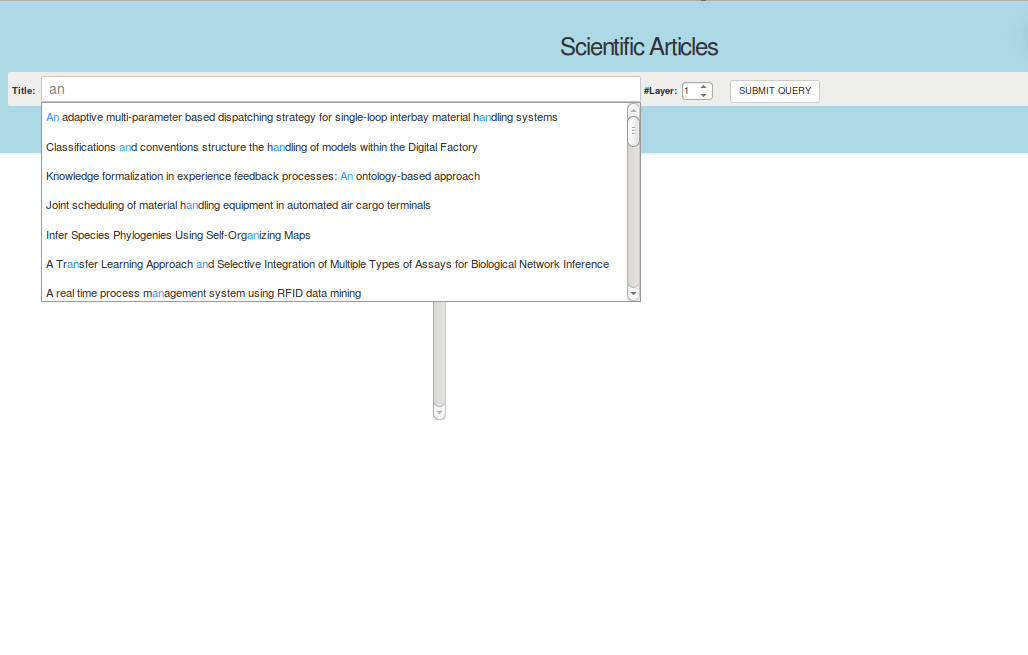
\includegraphics[scale=0.40]{immaginiTesina/vuoto.png}
\end{center}

La Search Bar \'e stata implementata in javascript (\textit{autocomplete.js}). I titoli degli articoli sono contenuti in un array che viene, ad ogni immissione, richiamato per mostrare i titoli che soddisfano la ricerca. Sottomessa la query, viene invocata la funzione \textit{generate-graph}. \newline \newline\newline
\lstinputlisting[style=java, firstline=189,lastline=263, caption=indexVisjs.html]{./WebSemanticoV2/indexVisjs.html}

\begin{center}
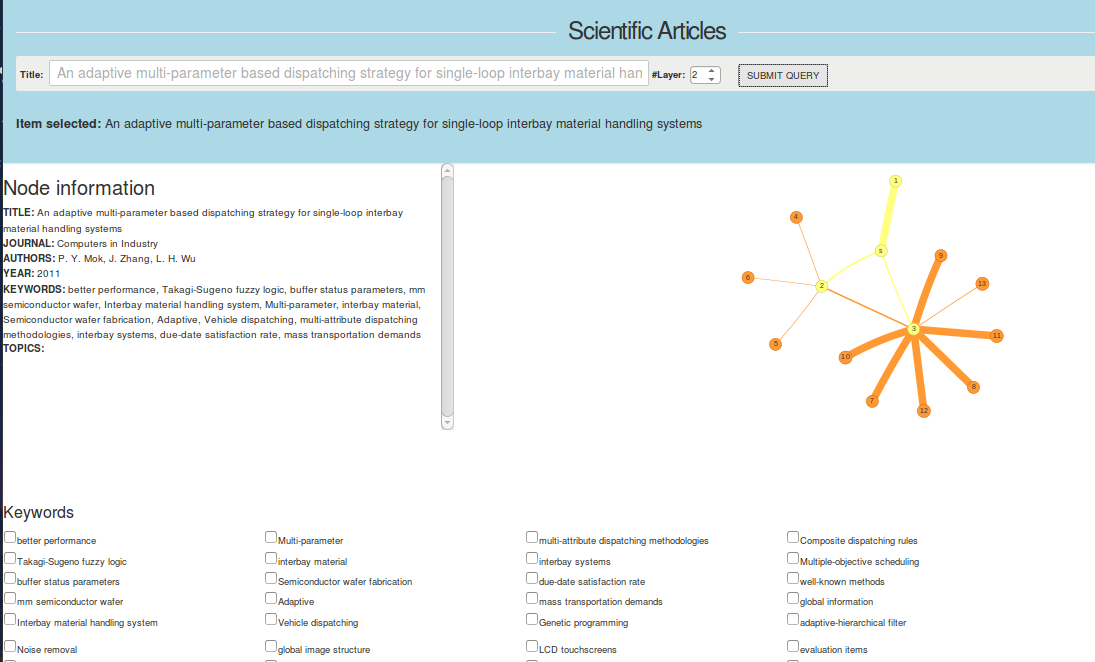
\includegraphics[scale=0.40]{immaginiTesina/2layer.png}
\end{center}


\section{Conclusioni}
\label{sec:conclusions}
Un altro utilizzo interessante, anche se non pienamente pertinente con gli obiettivi del lavoro, \'e la possibilit\'a di prevedere query che prendano in input dei topic e restituiscano tutti gli articoli che hanno quel topic e le relative parole chiave. In questo modo, cambiando il contesto (e.g. l'ontologia viene popolata con un set diverso di articoli, magari provenienti da una serie di conferenze), si pu\'o mostrare come lo stesso argomento viene trattato in maniera diversa a seconda del contesto. Se ad esempio il topic \'e \emph{Bioinformatica}, in un contesto di proceedings di conferenze informatiche le parole chiave potrebbero essere \emph{Algoritmi}, \emph{Strutture Dati}, \emph{Complessit\'a Computazionale}, etc. Mentre lo stesso topic in un contesto di proceedings di conferenze biologhe potrebbe avere come parole chiave \emph{Ribosomi}, \emph{Proteine}, etc. 





\end{document}
